\section{Problema 3}

\subsection{Enunciado}
El problema planteado consiste en encontrar un camino que un sapo deberá realizar en base a saltos entre piedras a diferente distancia, teniendo que llegar de una cierta piedra a otra, con la condicion de que cada salto tiene que estar en un rango de distancia.
La idea base del problema es encontrar el camino desde un vertice a otro de un grafo ponderado, sin necesidad de ser el camino minimo. 

\subsection{Soluci\'on}
La solución propuesta, al ser un problema común de grafos, es buscar el camino de un vertice a otro, y como no es necesario que sea el camino minimo usamos DFS (Busqueda en profundida), priorizando complejidad lineal en vez del mejor camino. Para esto, sabiendo que como maximo el sapo puede saltar 10 (o menos) piedras de un salto, generamos un grafo con todos los nodos, y luego agregamos las aristas de posible salto entre cada nodo, que como maximo podrián ser de 20.
Una vez generado el escenario, lo unico que queda es mediante el algoritmo DFS buscar el nodo final empezando por el inicio. 
En cada paso recursivo de la busqueda, marca como visitado el nodo actual, luego comprueba si el salto puede ser directo y termina la busqueda, en caso contrario, debera ir visitando los nodos adyacentes al nodo actual que aun no fueron visitados, de un maximo de 20, haciendo recursion con DFS en cada uno hasta encontrar el nodo final dando por finalizada la busqueda.
Es decir, usamos el algoritmo de DFS, pero le agregamos una optimizacion inicial para ciertos saltos donde el movimiento puede ser directo sin necesidad de seguir buscando un camino.

La correctitud del algoritmo queda demostrada por el hecho de que ya esta demostrada la correctitud del algoritmo de DFS.

\subsection{Pseudoc\'odigo}
\begin{codebox}
\Procname{$\proc{Resolver}$ (\textbf{in} $nodos$,\textbf{in} $x$,\textbf{in} $y$,\textbf{in} $p$,\textbf{in} $q$)}{pila}{Pila}
\li	\textbf{Si} el salto puede ser directo \Do \RComment O(1)
\li		return pila = (x,y); \End
\li	\textbf{Si no}  \Do
\li		grafo = Genero el grafo 				\RComment O(n)
\li		pila = Busco con DFS(grafo, inicio = x, fin = y)	\RComment O(n)\End 
\li	\textbf Devuelvo pila
\end{codebox}

\begin{codebox}
\Procname{$\proc{DFS}$ (\textbf{in} $grafo$,\textbf{in} $inicio$,\textbf{in} $fin$)}{pila}{Pila}
\li	\textbf{Si} el salto puede ser directo \Do 							\RComment O(1)
\li		return pila = (x,y); \End
\li	\textbf{Si no}  \Do
\li		Marco visitado al vértice \textit{inicio}						\RComment O(1)
\li		\textbf{Para} cada nodo adyacente del vértice \textit{inicio} \Do 	\RComment O(1)
\li			\textbf{Si} no fue visitado \Do \RComment O(1)
\li				\textbf{Si} es el vértice \textit{fin} que estoy buscando \Do \RComment O(1)	
\li					Agrego este vértice a la pila					\RComment O(1)
\li					Devuelvo la pila\End
\li				\textbf{Si no}  \Do
\li					Lo marco como visitado
\li					pila = Busco con DFS a partir de este nodo			\RComment O(n)
\li					Agrego este vértice a la pila
\li					Devuelvo la pila\End\End\End
\li	\textbf Devuelvo pila vacia
\end{codebox}

\subsection{Analisís de complejidad}	
El algoritmo consta de 2 etapas:\\ 

%\begin{itemsize}

Primero se genera el grafo, agregando todas las piedras como nodos, y uniendo cada nodo con aristas solamente si el salto es posible. Al haber n nodos, y por cada nodo un maximo de 20 aristas (ya que el salto maximo puede ser de 10 piedras cualquier \textit{dirección}), la complejidad final y sacando las constantes quedaría en O(n)\\  
Segundo, se debe buscar con el algoritmo de DFS desde el inicio hasta el fin, sin repetir los nodos ya visitados: O($|V|$ + $|E|$) = O(n + 10n) = O(n)\\  

%\end{itemsize}
Quedando como complejidad final O(n), tal como fue pedida. \\
\textit{Observación:} La cota minima de $\Omega$ $(1)$ se da en caso de que el salto pueda ser directo.

\subsection{Tests y Gráficos}
En el siguiente gráfico, con respecto a la cantidad de pie, se puede observar mediante la cantidad de ciclos que realizó el algoritmo para encontrar una solución, que la complejidad temporal del algoritmo es lineal a la cantidad de piedras.
\begin {center}
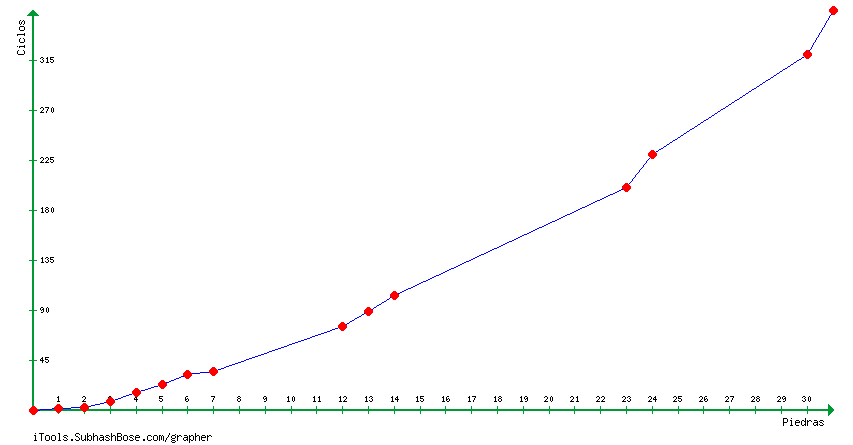
\includegraphics[width=15cm]{./graficos/grafico_ej3_0.png}
% grafico.eps: 0x0 pixel, 300dpi, 0.00x0.00 cm, bb=50 50 410 302
\end {center} 


\subsection{Conclusiones}
Como conclusión al problema dado en relación con la complejidad pedida, se puedo modelar un grafo de tal forma de encontrar un camino posible entre nodos, de modo tal que se priorice la performance temproal del algoritmo en vez de una solución más eficiente, ya que en caso contrario, si se quiere buscar un camino mínimo, la complejidad aumentaría considerablemente. 
